\chapter{Système d’acquisition}

\begin{figure}[h]
    \centering
    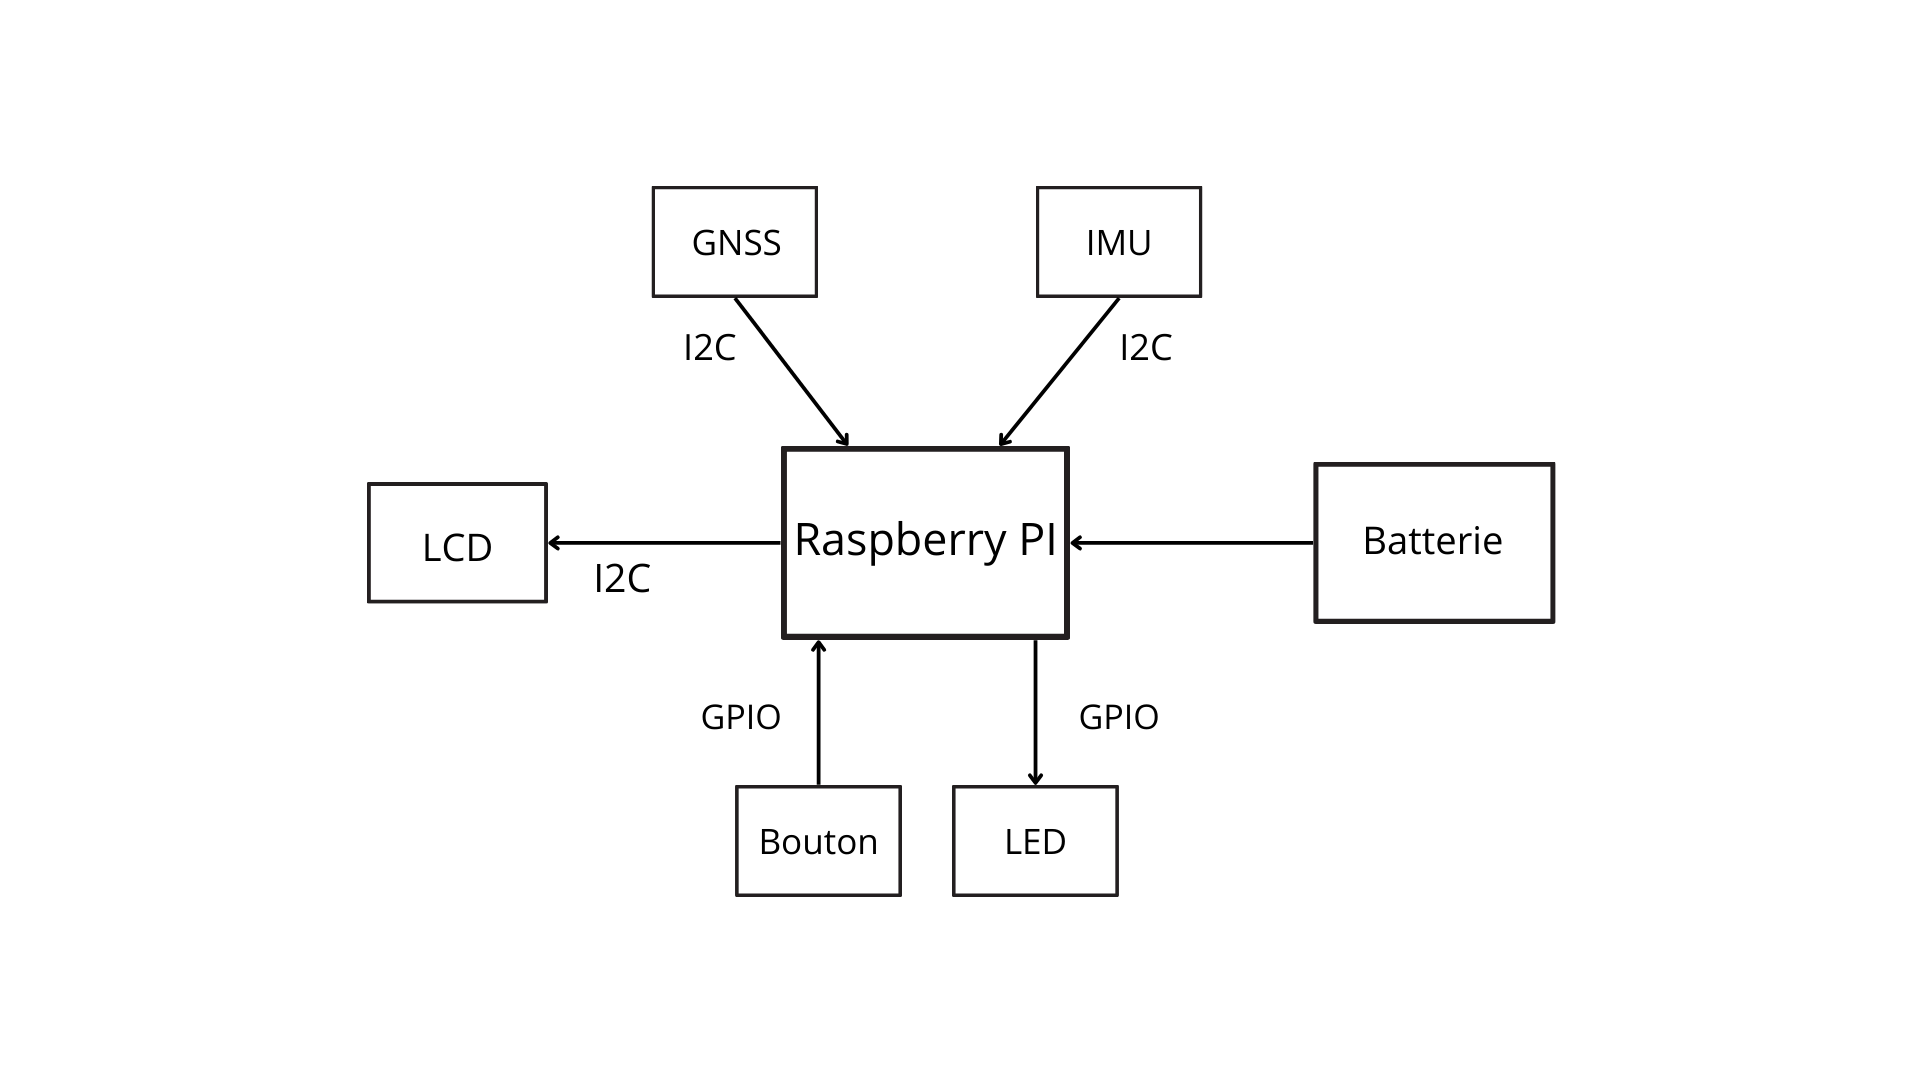
\includegraphics[width=1\textwidth]{montage.png} % nom de l'image et taille
    \caption{Figure 1 : Montage de notre RaspberryPI}
    \label{fig:montage}
\end{figure}

\section{Montage électronique et Description du système}

\vspace{1em}
\subsubsection*{Description globale du système}

Tout d'abord, le système est construit autour d’une Raspberry Pi 4 qui centralise les acquisitions des capteurs. Ceux-ci sont connectés via les ports GPIO et I2C, ce qui permet de faciliter la communication. Notre programme permet lancer l’acquisition à l'aide d'un bouton poussoir, une LED confirme alors le bon fonctionnement du système. Les données récupérées sont stockées localement et traitées directement avec la carte. Cela permet d'éviter toute manipulation des données par l'utilisateur. Après que les données aient été traitées, synchronisées, fusionnées et exploitées, le programme affiche la trajectoire sur OpenStreetMap.

\vspace{1em}
\subsubsection*{Chaine de traitement des données}

Afin de comprendre au mieux la façon dont nous avons construit notre système, voici les grandes étapes de notre algorithme :$\\$
Pression du Bouton poussoir $\Longrightarrow$ Acquisitions de l'IMU et du GNSS + LED allumée $\Longrightarrow$ Pression du Bouton poussoir $\Longrightarrow$ Prétraitement des valeurs aberrantes (rejets et remplacement) $\Longrightarrow$ Synchronisation temporelle des données du GNSS et de l'IMU $\Longrightarrow$ Conversion de la latitude et la longitude en coordonnées cartésiennes par rapport au centre de la Terre $\Longrightarrow$ Initialisation de la matrice de rotation de l'IMU $\Longrightarrow$ Suppression de l'erreur statique du gyroscope $\Longrightarrow$ Utilisation de la matrice de rotation + des données du gyroscope afin de changer la base de l'IMU $\Longrightarrow$ Utilisation des valeurs converties dans un filtre de Kalman $\Longrightarrow$ Reconversion des valeurs du GNSS en latitude et longitude $\Longrightarrow$ Affichage du trajet post-traitement.

\section{Choix des paramètres d’acquisition}
Comme nous l'avons précisé précédement, nous avons choisi de configurer nos capteurs afin qu'ils ne fournissent pas trop de données à traiter, tout en garantissant une bonne précision. Pour un humain qui marche ou qui court, il ne faut donc pas de grandes valeurs.

 Voici la liste des paramètres des capteurs:
\begin{itemize}
    \item \textbf{GNSS} : Fréquence d'acquisition à 1Hz
    \item \textbf{Accéléromètre} : Fréquence d'acquisition à 12.5Hz et plage de mesure à +/-2g.
    \item \textbf{Gyroscope} : Fréquence d'acquisition à 12.5Hz et plage de mesure à +/-2 dps.
    \item \textbf{Magnétomètre} : Fréquence d'acquisition à 40Hz et plage de mesure à 4 Gauss.
\end{itemize}

\vspace{1em}
\subsubsection*{Filtrage des signaux bruts}
Maintenant que nous avons determiné les paramètres d'acquisition, nous pouvons commencer à récupérer des données. Cependant, toutes les données ne sont pas exploitables. En effet, il est possible qu'il y ait des sauts de position. Pour cela, nous avons mis en place une méthode statistique afin de trier ces valeurs. Nous vous la présenterons alors dans la partie liées aux statistiques.

\section{Synchronisation des capteurs}
Après avoir récupéré nos données filtrées, il faut réussir à les sychroniser. C'est une étape cruciale, car cela nous permettera d'exploiter au mieux les différents types de données à un instant t. Plus précisément, cela nous permettera d'avoir un maximum d'information sur l'état du système à tout moment. Le problème qui se pose est que les capteurs, n'ont pas la même fréquence d'acquisition. Nous ne pouvons donc pas seulement les aligner directement sur une même échelle temporelle sans traitement préalable, car leurs données seraient désynchronisées et pourraient induire des erreurs d’interprétation.

Dans cette partie, nous vous présenterons alors comment nous avons aligner nos données de manière temporelle. En ce qui concerne l'alignement spatial, nous en parlerons plus tard.

Dans un premier temps, il nous a fallu synchroniser les données du GNSS avec celles du téléphone. Pour cela, nous avons travaillé avec le TimeStamp du GPS ainsi que les heures d'acquisitions du téléphone. Sachant que le GNSS et le téléphone donnent une mesure chaque seconde, il n'était pas difficile de les synchroniser. Nous avons alors rogné l'ensemble des données disponibles selon le min et le max (de la date) de chaque plage de données.
Finalement, cette synchronisation nous a permis de comparer les valeurs du GNSS sans traitement avec des valeurs "réelles" et ainsi determiner l'erreur statique.

Dans un second temps, nous avons synchronisé les données du GNSS avec celles de l'IMU. C'est une tâche plus difficile car les fréquences d'acquisitions sont différentes. Nous avons alors séparé ce traitement en deux parties:
\begin{itemize}
    \item \textbf{Réduction des plages de données} : Comme précédemment, nous avons rogné l'ensemble des données disponibles selon le min et le max (du TimeStamp) de chaque plage de données.
    \item \textbf{Interpolation linéaire} : Afin d'avoir un maximum de données exploitables, au lieux de supprimer l'excès de valeurs de l'IMU, nous avons prédit les valeurs associées pour le GNSS.
\end{itemize}
Finalement, ce traitement nous permettera d'utiliser les données dans la partie fusion de données.

